\documentclass[12pt]{article}

\usepackage{graphicx}
\usepackage{colortbl}
\usepackage{xr}
\usepackage{hyperref}
\usepackage{longtable}
\usepackage{xfrac}
\usepackage{tabularx}
\usepackage{array,ragged2e}
\usepackage{float}
\usepackage{booktabs}
\usepackage{caption}
\usepackage{pdflscape}
\usepackage{afterpage}
\usepackage{tabu}
\usepackage{multirow}
\usepackage{geometry}

\usepackage[round]{natbib}

%\usepackage{refcheck}

\hypersetup{
    bookmarks=true,         % show bookmarks bar?
      colorlinks=true,       % false: boxed links; true: colored links
    linkcolor=red,          % color of internal links (change box color with linkbordercolor)
    citecolor=green,        % color of links to bibliography
    filecolor=magenta,      % color of file links
    urlcolor=cyan           % color of external links
}

%% Comments

\usepackage{color}

\newif\ifcomments\commentstrue %displays comments
\newif\ifcomments\commentsfalse %so that comments do not display

\ifcomments
\newcommand{\authornote}[3]{\textcolor{#1}{[#3 ---#2]}}
\newcommand{\todo}[1]{\textcolor{red}{[TODO: #1]}}
\else
\newcommand{\authornote}[3]{}
\newcommand{\todo}[1]{}
\fi

\newcommand{\wss}[1]{\authornote{blue}{SS}{#1}} 
\newcommand{\plt}[1]{\authornote{magenta}{TPLT}{#1}} %For explanation of the template
\newcommand{\an}[1]{\authornote{cyan}{Author}{#1}}

%% Common Parts

\newcommand{\progname}{Sayyara} % PUT YOUR PROGRAM NAME HERE
\newcommand{\authname}{Team 31
\\ SFWRENG 4G06
\\ Christopher Andrade
\\ Alyssa Tunney
\\ Kai Zhu
\\ Ethan Vince-Budan
\\ Collin Kan
\\ Harsh Gupta} % AUTHOR NAMES                  

\usepackage{hyperref}
    \hypersetup{colorlinks=true, linkcolor=blue, citecolor=blue, filecolor=blue,
                urlcolor=blue, unicode=false}
    \urlstyle{same}

% For easy change of table widths
\newcommand{\colZwidth}{1.0\textwidth}
\newcommand{\colAwidth}{0.13\textwidth}
\newcommand{\colBwidth}{0.82\textwidth}
\newcommand{\colCwidth}{0.1\textwidth}
\newcommand{\colDwidth}{0.05\textwidth}
\newcommand{\colEwidth}{0.8\textwidth}
\newcommand{\colFwidth}{0.17\textwidth}
\newcommand{\colGwidth}{0.5\textwidth}
\newcommand{\colHwidth}{0.28\textwidth}

% Used so that cross-references have a meaningful prefix
\newcounter{defnum} %Definition Number
\newcommand{\dthedefnum}{GD\thedefnum}
\newcommand{\dref}[1]{GD\ref{#1}}
\newcounter{datadefnum} %Datadefinition Number
\newcommand{\ddthedatadefnum}{DD\thedatadefnum}
\newcommand{\ddref}[1]{DD\ref{#1}}
\newcounter{theorynum} %Theory Number
\newcommand{\tthetheorynum}{T\thetheorynum}
\newcommand{\tref}[1]{T\ref{#1}}
\newcounter{tablenum} %Table Number
\newcommand{\tbthetablenum}{T\thetablenum}
\newcommand{\tbref}[1]{TB\ref{#1}}
\newcounter{assumpnum} %Assumption Number
\newcommand{\atheassumpnum}{P\theassumpnum}
\newcommand{\aref}[1]{A\ref{#1}}
\newcounter{goalnum} %Goal Number
\newcommand{\gthegoalnum}{P\thegoalnum}
\newcommand{\gsref}[1]{GS\ref{#1}}
\newcounter{instnum} %Instance Number
\newcommand{\itheinstnum}{IM\theinstnum}
\newcommand{\iref}[1]{IM\ref{#1}}
\newcounter{usecasenum} %Use Case Number
\newcommand{\rtheusecasenum}{UC\theusecaseum}
\newcounter{authreqnum} %Authentication Requirement Number
\newcommand{\rtheauthreqnum}{AuR\theauthreqnum}
\newcommand{\authref}[1]{AuR\ref{#1}}
\newcounter{servicereqnum} %Service Requirement Number
\newcommand{\rtheservicereqnum}{SR\theservicereqnum}
\newcommand{\serviceref}[1]{SR\ref{#1}}
\newcounter{parreqnum} %Profile and Analytic Requirement Number
\newcommand{\rtheparreqnum}{PAR\theparreqnum}
\newcommand{\parref}[1]{PAR\ref{#1}}
\newcounter{appreqnum} %Appointment Requirement Number
\newcommand{\rtheappreqnum}{P\theappreqnum}
\newcommand{\appref}[1]{ApR\ref{#1}}
\newcounter{workreqnum} %Work Order Requirement Number
\newcommand{\rtheworkreqnum}{P\theworkreqnum}
\newcommand{\workref}[1]{WOR\ref{#1}}
\newcounter{quotereqnum} %Quote Requirement Number
\newcommand{\rthequotereqnum}{P\thequotereqnum}
\newcommand{\quoteref}[1]{QR\ref{#1}}
\newcounter{searchreqnum} %Quote Requirement Number
\newcommand{\rthesearchreqnum}{P\thesearchreqnum}
\newcommand{\searchref}[1]{SLR\ref{#1}}
\newcounter{vendorreqnum} %Vendor Requirement Number
\newcommand{\rthevendorreqnum}{VR\thevendorreqnum}
\newcommand{\vendorref}[1]{VR\ref{#1}}
\newcounter{lfrnum} %Look and Feel Requirement Number
\newcommand{\rthelfrnum}{LFR\thelfrnum}
\newcommand{\lfrref}[1]{LFR\ref{#1}}
\newcounter{uhrnum} %Usability and Humanity Requirement Number
\newcommand{\rtheuhrnum}{UHR\theuhrnum}
\newcommand{\uhrref}[1]{UHR\ref{#1}}
\newcounter{prnum} %Performance Requirement Number
\newcommand{\rtheprnum}{PR\theprnum}
\newcommand{\prref}[1]{PR\ref{#1}}
\newcounter{oernum} %Operational and Environmental Requirement Number
\newcommand{\rtheoernum}{OER\theoernum}
\newcommand{\nfrref}[1]{OER\ref{#1}}
\newcounter{msrnum} %Maintainability and Support Requirement Number
\newcommand{\rthemsrnum}{MSR\themsrnum}
\newcommand{\msrref}[1]{MSR\ref{#1}}
\newcounter{srnum} %Security Requirement Number
\newcommand{\rthesrnum}{SR\thesrnum}
\newcommand{\srref}[1]{SR\ref{#1}}
\newcounter{cprnum} %Cultural and Political Requirement Number
\newcommand{\rthecprnum}{CPR\thecprnum}
\newcommand{\cprref}[1]{CPR\ref{#1}}
\newcounter{crnum} %Compliance Requirement Number
\newcommand{\rthecrnum}{CR\thecrnum}
\newcommand{\crref}[1]{CR\ref{#1}}
\newcounter{lcnum} %Likely change number
\newcommand{\lthelcnum}{LC\thelcnum}
\newcommand{\lcref}[1]{LC\ref{#1}}
\newcounter{ucnum} %Unlikely change number
\newcommand{\ltheucnum}{UC\theucnum}
\newcommand{\ucref}[1]{UC\ref{#1}}

\usepackage{fullpage}

\newcommand{\deftheory}[9][Not Applicable]
{
\newpage
\noindent \rule{\textwidth}{0.5mm}

\paragraph{RefName: } \textbf{#2} \phantomsection 
\label{#2}

\paragraph{Label:} #3

\noindent \rule{\textwidth}{0.5mm}

\paragraph{Equation:}

#4

\paragraph{Description:}

#5

\paragraph{Notes:}

#6

\paragraph{Source:}

#7

\paragraph{Ref.\ By:}

#8

\paragraph{Preconditions for \hyperref[#2]{#2}:}
\label{#2_precond}

#9

\paragraph{Derivation for \hyperref[#2]{#2}:}
\label{#2_deriv}

#1

\noindent \rule{\textwidth}{0.5mm}

}

\newcommand{\rev}[1]{(\textit{Planned for Rev#1})}

\begin{document}

\title{Software Requirements Specification for \progname: A Progressive Web Application for the Automotive Industry} 
\author{\authname}
\date{\today}
	
\maketitle

~\newpage

\pagenumbering{roman}

\section*{Revision History}

\begin{table}[hp]
    \begin{tabularx}{\textwidth}{p{3cm}p{2cm}X}
    \toprule {\bf Date} & {\bf Version} & {\bf Notes}\\
    \midrule
    Sept. 29, 2022 & 0.0 & Adaptation of Volere template\\
    Oct. 4, 2022 & 0.5 & Preliminary draft\\
    Oct. 5, 2022 & 1 & Final version of revision 0\\
    April 5, 2023 & 1 & Revision 1\\
    \bottomrule
    \end{tabularx}\\ \\
    \caption{Revision History}
\end{table}

\noindent The team is using the Volere template for this SRS.\\
Adapted from: https://www.volere.org/templates/volere-requirements-specification-template/

~\newpage

\tableofcontents

\listoftables

\listoffigures

~\newpage

\section{Introduction}
This document outlines the stakeholders, requirements, and potential issues in 
developing a progressive web application for the automotive industry. 
The document will serve as a guide for for upcoming design stages, and will 
also provide the stakeholders with a high level description of the application.
The requirements listed in this document will be consulted for validation of
features during development, and to ensure that the scope matches the client's
expectations.

\subsection{The User Business or Background of the Project Effort}
Automobile maintenance and repairs are an unavoidable and recurring part of any
car owner's experience. Despite its ubiquity, acquiring professional auto
service remains a time-consuming and hassle-prone process. Without a systemic
procedure, this process consists of a number of scattered and repetitive tasks,
beginning with finding local providers including mechanics, tire shops, and
body shops through traditional means such as a search engine, with little
assurance of the trustworthiness or service quality of the providers in the
search results.

After obtaining a list of service providers, customers are required to contact
each service professional separately, repeatedly describing the same problems
in order to receive a quote.  Furthermore, different providers may have
different availability. Scheduling a time preferred by the customer at
available auto service providers, therefore, requires further communication
with multiple providers through methods such as phone or in-person visits,
costing additional time and effort.

\section{Goals of the Project}
To address these problems in the auto service industry, The team seeks to deliver
an all-in-one tool that connects customers with auto shop owners and employees for 
frequent tasks such as service inquiries, quotes, and scheduling.

    \begin{itemize}
        \item[G\refstepcounter{goalnum}\thegoalnum \label{R_Output}.] Allow vehicle owners to find automotive service providers based on personal criteria (location, availability, offered services, customer ratings, etc.)

        \item[G\refstepcounter{goalnum}\thegoalnum \label{R_Output}.] Allow automotive service providers to easily get an online presence and increase their customer base.

        \item[G\refstepcounter{goalnum}\thegoalnum \label{R_Output}.] Allow vehicle owners to save time by getting quotes for service on their car from multiple auto shops at a time.

        \item[G\refstepcounter{goalnum}\thegoalnum \label{R_Output}.] Allow automotive service providers to digitize their records.

        \item[G\refstepcounter{goalnum}\thegoalnum \label{R_Output}.] Allow vehicle owners to flexibly schedule their service based on the availability of their desired automotive service provider.

        \item[G\refstepcounter{goalnum}\thegoalnum \label{R_Output}.] Allow automotive service providers to more effectively schedule the use of resources such as vehicle bays and employees.

        \item[G\refstepcounter{goalnum}\thegoalnum \label{R_Output}.] Allow quick communication between vehicle owners and automotive shops for topics such as providing estimates, asking questions or giving general updates on service.

        \item[G\refstepcounter{goalnum}\thegoalnum \label{R_Output}.] Allow vehicle owners to maintain digital records of servicing their vehicle including inspection results, invoices and appointment records.

        \item[G\refstepcounter{goalnum}\thegoalnum \label{R_Output}.] Provide individuals with no background in website/online management a simple and satisfying experience working digitally.
    \end{itemize}

\section{Stakeholders}
\subsection{The Client}
Nabil Ibrahim of Sayyara is the project sponsor and supervisor who stipulates
the scope of the project and verifies the deliverables.
\subsection{The Customers}
Owners of automotive service shops, including body shops, tire shops, and
independent mechanics are the intended customers of the product. The owners
will acquire the license to use the software on behalf of employees and their
potential customers.
\subsection{The Other Stakeholders}
\subsubsection{Developers}
Members of Team 31 are the developers of the application, responsible for the
design, implementation, and testing of the software.
\subsubsection{Capstone Staff}
Dr. Spencer Smith, the instructor of the Software Engineering capstone course
at McMaster University, and his team of teaching assistants are advisors who
provide evaluation and feedback of project deliverables.
\subsubsection{Automotive Part Vendors}
Car part vendors may have a stake in the project as the process of streamlining
auto service client-provider interactions may also include ordering parts
directly or indirectly through the application.

\subsection{The Hands-On Users of the Product}
\subsubsection{Automotive Shop Owners}
Shop owners are responsible for the initial setup of the shop profile in the
application. They may also use the application to monitor performance related
metrics such as customer volume and service statistics. The owners may have
limited experience with web applications, but should at minimum have access to
a computer or mobile device.

\subsubsection{Automotive Shop Employees}
Shop employees are a group of primary users of the software, who interact with
customers through the application to provide services. Employees are adults of
all ages with limited to moderate levels of experience in using web 
applications.

\subsubsection{Automobile Owners}
Car owners are the main group of intended users, who can use the application
to connect to auto shops and schedule for services. There is great diversity in
the age, knowledge, and background among the customers, thus all levels of
technological experience can be expected. At the minimum, they must have 
access to a computer or mobile device with an Internet connection, and have
some previous experience in using the device.

\subsection{Personas}
N/A
\subsection{Priorities Assigned to Users}
N/A
\subsection{User Participation}
Users, regardless of whether it is an automotive shop owner, employee, or customer, will be required to fill out a few forms when they are interacting
with the website. These forms will be as as minimal and simplistic as possible to ensure that users do not get frustrated and exit the application
halfway through what they are working on. Since it is expected that users may not have much technology experience, this process will be made as
comfortable as possible for them.

\subsection{Maintenance Users and Service Technicians}
Team 31 will be the primary maintenance users of the system since they are the developers and will have the most knowledge to debug and fix any issues.
Additional workers may need to be hired on at a later date to assist with maintenance depending on the final scope and outcomes of the project.

\section{Project Constraints}
\subsection{Solution Constraints}
\begin{itemize}
    \item The final product must be a PWA.
    \item The final product must be fully functional and usable by all potential user types.
    \item The final product must be fully functional on desktop devices.
\end{itemize}

\subsection{Implementation Environment and the Current System}
\begin{itemize}
    % \item Because the final product needs to be a PWA, it needs to be hosted on a web server.
    \item The final product must be connected to a database that can encrypt and store user information.
    \item The final product must be developed with both a front-end and a back-end.
\end{itemize}

\subsection{Partner or Collaborative Applications}
N/A
\subsection{Off-the-Shelf Software}
\begin{itemize}
    \item Database software
    \item Front-end frameworks and libraries
    \item Payment authentication system
    % \item Web server platform as a service
\end{itemize}

\subsection{Anticipated Workplace Environment}
The anticipated workplace environment where the product is expected to be used will be in automotive vehicle shops. The application will be used to make automotive shop owners' and employees' various tasks more efficient.

\subsection{Schedule Constraints}
\begin{itemize}
    \item End of March 2023 - Final demonstration of finished product due
    \item April 5, 2023 - Final documentation for product due
\end{itemize}
\subsection{Budget Constraints}
\begin{itemize}
    \item \$750 total budget (database and web hosting will be a cost)
\end{itemize}
\subsection{Enterprise Constraints}
N/A

\section{Naming Conventions and Terminology}
\subsection{Glossary of All Terms, Including Acronyms, Used by Stakeholders involved in the Project}
\subsubsection{Stakeholder Naming}
\renewcommand{\arraystretch}{1.2}
\begin{table}[H]
    \begin{tabularx}{\textwidth}{l X}
        \toprule
        \textbf{Term} & \textbf{Meaning} \\
        \midrule
        User & Any individual directly interacting with the system.\\
        Shop Owner & A User who has administrative authority over an automotive shop.\\
        Employee & A User working under a Shop Owner.\\
        Vehicle Owner/Customer & A User responsible for a vehicle which may need servicing.\\ % dont like this def but its ok
        \bottomrule
    \end{tabularx} \\ \\
    \caption{Stakeholder Naming}
\end{table}

\subsubsection{Other Terms}
\begin{table}[H]
    \begin{tabularx}{\textwidth}{l X}
        \toprule
        \textbf{Term} & \textbf{Meaning} \\
        \midrule
        Business & An automotive service provider.\\
        % OBD2 Sensor & A tool used to show what is going on inside a vehicle and can help avoid any costly unnecessary repairs.\\
        PWA & Progressive Web Application - an application that can natively run on both desktop and mobile browsers without the need for an external application.\\
        POC & The proof of concept is a low fidelity demonstration of a few core functions displayed on a skeletal front end.\\
        MVP & The minimum viable product is the project deliverable by the end of the capstone development phase containing the core features as requested by the client.\\
        \bottomrule
    \end{tabularx} \\ \\
    \caption{Other Terms}
\end{table}

\section{Relevant Facts and Assumptions}

\subsection{Relevant Facts}

\begin{itemize}
    \item The product is being specifically designed for use in the automotive industry.
    \item Currently in the automotive industry, 
    \begin{itemize}
        \item Shop owners cannot scale their businesses or retain customers long term as they are unable to compete with dealers when it comes to convenience, availability, and trust.
        \item Shop owners cannot provide accurate time estimates as to when they can work on servicing a customer's vehicle.
        \item Shop owners have a hard time answering all the calls they get on a daily basis.
        \item Customers have a fear of being overcharged.
        \item Customers have to endure a cumbersome process to obtain quotes and book service appointments.
        \item Customers have no digital trail of the work performed on their vehicle.
    \end{itemize}
\end{itemize}

\subsection{Business Rules}
N/A

\subsection{Assumptions}
\begin{itemize}
    \item All users own a computer.
    \item All users have a basic understanding of how to use a computer.
    \item All users have a basic understanding of how to use a web browser.
    \item All customers own a vehicle.
\end{itemize}

\section{The Scope of the Work}

\subsection{The Current Situation}

There is currently no application or service that easily presents a customer, who needs to service their vehicle, with a network of automotive businesses and the option to easily view the businesses' schedules and book an appointment. We will build such a service, where the customer will also have the option to describe their issue in detail and receive a quote from the variety of businesses before committing to any one business. The main service, which will be seen and used by the users, which include vehicles owner, shop owners, and shop employees, will be a PWA. The service is built with the front-end framework React and TypeScript, while the back-end is built using Python. The user database and appointment information are managed by Supabase. 
\subsection{The Context of the Work}

\begin{figure}[H]
    \centering
    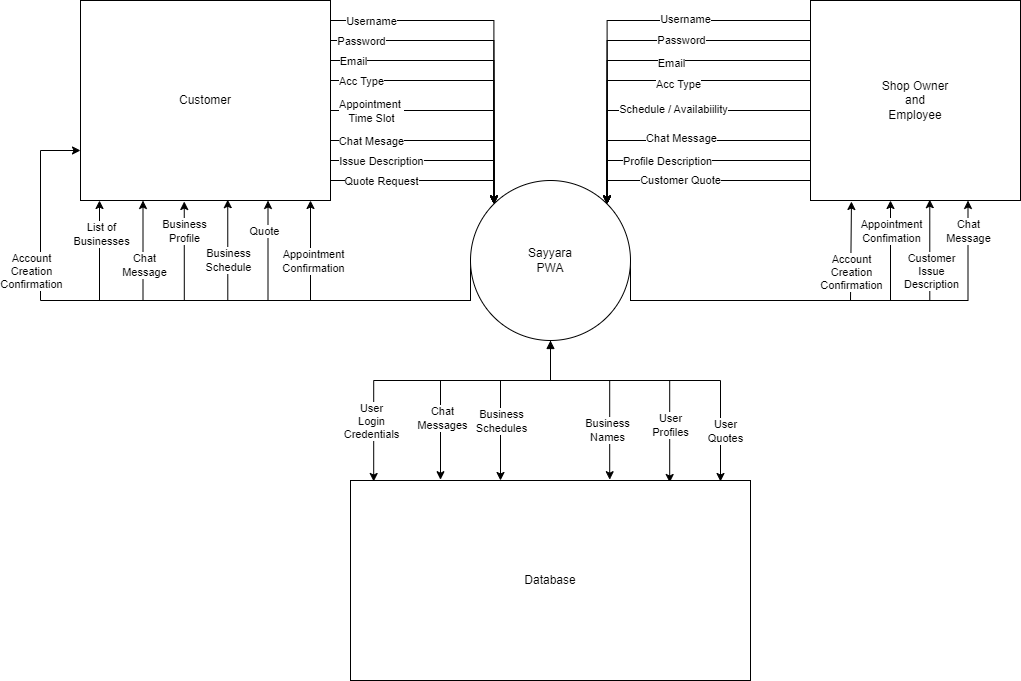
\includegraphics[scale=0.5]{SRS/wcd.png}
    \caption{Work Context Diagram}
    \label{fig:wcd}
\end{figure}

\subsection{Work Partitioning}
% TODO: Add phase in plan

\newcolumntype{P}[1]{>{\RaggedRight\arraybackslash}p{#1}}
\renewcommand{\arraystretch}{1.2}
\begin{longtable}{| l | P{3.3cm} | P{4.7cm} | P{7cm} |} 
    \hline
    \textbf{No.} & \textbf{Event Name} & \textbf{Input and Output} & \textbf{Summary}\\
    \hline \hline
% # & EVENT NAME &
    % \begin{tabular}{P{4.5cm}}\\
    % IN/OUT\\
    % IN/OUT\\
    % \end{tabular} &
    % EVENT SUMMARY\\
    % \hline
    
    1 & User creates account &
    \begin{tabular}{P{4.5cm}}\\
    User Type (IN)\\
    User Name (IN)\\
    User Password (IN)\\
    Email (IN)\\
    Confirmation (OUT)\\
    \end{tabular} &
    User will be able to sign up to create an account by providing a username and password. User will also be able to choose which type of user they are (e.g. Customer, Shop Owner, Employee)\\
    \hline
    
    2 & User logs in & 
    \begin{tabular}{P{4.5cm}}\\
    User Name (IN)\\
    User Password (IN)\\
    \end{tabular} & 
    User logs into the app with their chosen username and password.\\
    \hline
    
    3 & Customer requests a quote & 
    \begin{tabular}{P{4.5cm}}\\
    User Info (IN)\\
    Issue Description (IN)\\
    Quote(s) (OUT)\\
    \end{tabular} & 
    Customer describes their issue in detail and requests and quote. They will receive a quote from any interested shop owners.\\
    \hline
    
    4 & Customer views businesses &
    \begin{tabular}{P{4.5cm}}\\
    Businesses List (OUT)\\
    \end{tabular} &
    Customer will be able to view the list of currently available businesses where they can service their vehicle.\\
    \hline
    
    5 & Customer views schedule &
    \begin{tabular}{P{4.5cm}}\\
    Business Name (IN)\\
    Schedule (OUT)\\
    \end{tabular} &
    Customer can click on a business to view its current schedule.\\
    \hline

    6 & Owner or Employee views schedule &
    \begin{tabular}{P{4.5cm}}\\
    Time Slots (IN)\\
    Schedule (OUT)\\
    \end{tabular} &
    Show owners and employees will be able to view their own schedule to view any appointments and will also be able to edit their availability.
    \hline
    
    7 & Customer books an appointment &
    \begin{tabular}{P{4.5cm}}\\
    Time Slot (IN)\\
    Confirmation (OUT)\\
    \end{tabular} &
    Customers will be able to select a time slot from a given schedule to book and appointment. The customer, shop owner, and employee will then be given a confirmation receipt of the customer's appointment.\\
    \hline

    8 & User chat &
    \begin{tabular}{P{4.5cm}}
    User1 Message (IN)\\
    User2 Response (OUT)\\
    \end{tabular} &
    Two users, a customer and a shop owner/employee will be able to chat with one another to further discuss the customer's vehicle problems and other details.\\
    \hline
    
    9 & User Profile &
    \begin{tabular}{P{4.5cm}}\\
    Description (IN)\\
    \end{tabular} &
    Shop owners and employees can go to their profile page to update their own descriptions.\\
    \hline

    10 & User Search &
    \begin{tabular}{P{4.5cm}}\\
    Shop Search Query (IN)\\
    Shop Search Results (OUT)\\
    \end{tabular} &
    Vehicle Owners will be able to search for shops registered to the system by name or by address. Additionally, they can apply filters to further refine the search results. They can then perform a number of quick actions from the search list.\\
    \hline
    
    \caption{Work Partitioning}
\end{longtable}

\subsection{Specifying a Business Use Case (BUC)}


\\ \textbf{Business Event 1}: User wants to create an account
\\ \textbf{Business Use Case}: Create a user account
\\ \textbf{Trigger}: Account Creation Request
\\ \textbf{Preconditions}: None
\\ \textbf{Interested Stakeholders}: Developers, Maintainers
\\ \textbf{Active Stakeholders}: Customer, Shop Owner, Employee
\\ - The User requests to create an account
\\ - The User will be prompted to choose their account type and for a username, password, and email
\\ - The system will create the account if the given username is not taken
\\ - The User will receive an account creation confirmation


\\ \textbf{Business Event 2}: User wants to log in
\\ \textbf{Business Use Case}: User will be authenticated by the system
\\ \textbf{Trigger}: Login Request
\\ \textbf{Preconditions}: User has created an account
\\ \textbf{Interested Stakeholders}: Developers, Maintainers
\\ \textbf{Active Stakeholders}: Customer, Shop Owner, Employee
\\ - The User will request to log in
\\ - The User will provide their username and password
\\ - If the credentials are exist and are correct, the user will be logged in
\\ - If not, the user will be notified that the username or password is incorrect
\\

\\ \textbf{Business Event 3}: Customer wants to request a quote
\\ \textbf{Business Use Case}: Shop Owner or Employee provides a customer quote
\\ \textbf{Trigger}: Quote Request
\\ \textbf{Preconditions}: User must provide a detailed  explanation of their vehicle issue
\\ \textbf{Interested Stakeholders}: Developers, Maintainers
\\ \textbf{Active Stakeholders}: Customer, Shop Owner, Employee
\\ - Customer will first provide a detailed description of the issue their vehicle is encountering
\\ - Willing Shop Owners and Employees will review the description, diagnose the issue, and then provide the customer with a quote
\\

\\ \textbf{Business Event 4}: Customer wants a list of the available businesses
\\ \textbf{Business Use Case}: Provide a list of participating businesses 
\\ \textbf{Trigger}: Business List Request
\\ \textbf{Preconditions}: There must be at least one available business
\\ \textbf{Interested Stakeholders}: Shop Owner, Employee, Developers, Maintainers
\\ \textbf{Active Stakeholders}: Customer
\\ - Customer will click on the shop lookup page
\\ - System will provide the customer with a list of all participating businesses.
\\ - Customer can search through this list and filter the results.
\\

\\ \textbf{Business Event 5}: Customer wants to views the schedules of a certain business
\\ \textbf{Business Use Case}: Provide a certain business' schedule
\\ \textbf{Trigger}: View Schedule Request
\\ \textbf{Preconditions}: There must be at least one available business that filled out their availability
\\ \textbf{Interested Stakeholders}: Shop Owner, Employee, Developers, Maintainers
\\ \textbf{Active Stakeholders}: Customer
\\ - Customer will click on a business from a list of participating businesses
\\ - Customer will be provided with a description of the business and their schedule / availability
\\

\\ \textbf{Business Event 6}: Shop Owners or Employees wants to view or edit their schedules
\\ \textbf{Business Use Case}: Display and/or edit schedule
\\ \textbf{Trigger}: View Schedule Request
\\ \textbf{Preconditions}: Must be logged into a shop owner or employee account
\\ \textbf{Interested Stakeholders}: Customer, Developers, Maintainers
\\ \textbf{Active Stakeholders}: Shop Owner, Employee
\\ - Shop Owner or Employee clicks on their profile
\\ - User will be able to view their schedule as a customer might see it
\\ - User can edit the schedule by filling out time slots in which they are available or unavailable
\\ - System will make the corresponding changes to their schedule
\\

\\ \textbf{Business Event 7}: Customers wants to book and appointments
\\ \textbf{Business Use Case}: Create an appointment
\\ \textbf{Trigger}: Appointment Creation Request
\\ \textbf{Preconditions}: Appointment time slot is available, user is logged in
\\ \textbf{Interested Stakeholders}: Developers, Maintainers
\\ \textbf{Active Stakeholders}: Customer, Shop Owner, Employee
\\ - Customer will be able to provide a business a time slot that is available
\\ - System will keep track of the time slot, and update Shop Owner and Employee's schedules as unavailable
\\ - Customer, Shop Owner, and Employee will each receive a confirmation of the appointment
\\ - Employee will receive a confirmation if they were available during the appointment
\\

\\ \textbf{Business Event 8}: User wants to chat with another user
\\ \textbf{Business Use Case}: Send user message to target user
\\ \textbf{Trigger}: Chat Request
\\ \textbf{Preconditions}: User must be logged in
\\ \textbf{Interested Stakeholders}: Developers, Maintainers
\\ \textbf{Active Stakeholders}: Customer, Shop Owner, Employee
\\ - User will have an option to message another user
\\ - Chat can only be created between a Customer and Shop Owner/Employee and vice versa
\\ - User will input their message and send
\\ - System will log the message and send to the receiving user 
\\

\\ \textbf{Business Event 9}: User wants to view or update their personal profile
\\ \textbf{Business Use Case}: Update Personal Profile
\\ \textbf{Trigger}: View Profile Request
\\ \textbf{Preconditions}: User must be logged in
\\ \textbf{Interested Stakeholders}: Customer, Developers, Maintainers
\\ \textbf{Active Stakeholders}: Shop Owner, Employee
\\ - Shop Owner or Employee clicks on their profile
\\ - User will be able to view their profile as a customer might see it
\\ - User will be able to edit their profile description by providing an updated description.
\\ - System will make the corresponding changes to their profile


\section{Business Data Model and Data Dictionary}

\begin{figure}[H]
    \centering
    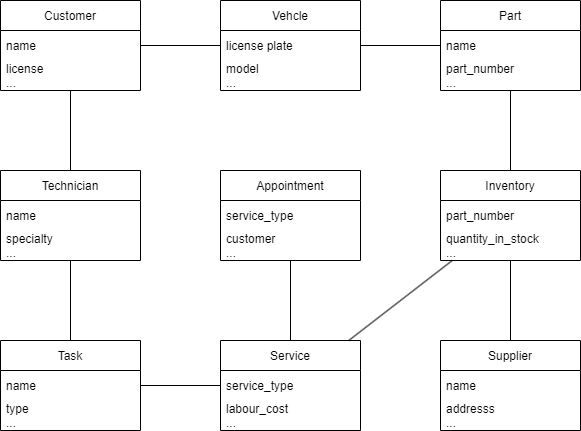
\includegraphics[scale=0.7]{dmd.drawio}
    \caption{Business data model for Sayyara}
    \label{fig:bdm}
\end{figure}

\subsection{Business Data Model}
The business data model illustrated in figure\ref{fig:bdm} defines the foundational entities and associations used in the automotive repair shop. Vehicles are owned by customers and are brought in to be serviced. Vehicles that are serviced are assigned a service order by the service bay manager or generally the owner. A repair shop technician is assigned to the service order. The technician inspects the car and makes repairs to the car. The technician keeps a detailed record of the repairs made on the car, which are routed back to the customer.

\textbf{Note} that the data models related to Inventory, Supplier and Part are a part of the extended goals in the our scope of work and will not be a part of the MVP or POC demo.
\pagebreak
\subsection{Data Dictionary}

The data dictionary below outlines a brief overview of the data flowing through the PWA. The following classes provide the atomic data classes to build the PWA.

\\

\renewcommand{\arraystretch}{1.2}
\begin{longtable}{p{3cm}p{10cm}p{2cm}}
    \toprule
    \textbf{Name} & \textbf{Content}    & \textbf{Type} \\ 
    \midrule
    Customer      & Customer ID         & Class         \\
    Vehicle       & Vehicle Details & Class         \\
    Technician    & Name                & Class         \\
    Service       & Service Type + Service Cost         & Class         \\
    Task          & Task Name + Task Type         & Class         \\
    Appointment   & Customer ID + Vehicle + Service + Appointment &  Class \\
    \bottomrule
    \caption{Data Dictionary Table 1}
\end{longtable}


\renewcommand{\arraystretch}{1.2}
\begin{longtable}{p{4cm}p{10cm}p{2cm}}
    \toprule
    \textbf{Name} & \textbf{Content}    & \textbf{Type} \\ 
    \midrule
    Vehicle Details & \{License Plate + VIN  + Make, Model, Year\}    & Attribute         \\
    Customer ID     & hash(Customer Name + License Number)         & Attribute         \\
    Customer Name     & *from Customer*         & Attribute         \\
    License Number     &    *from Customer*      & Attribute         \\
    Technician Specialty  &      *Specialization of the technician*    & Attribute         \\
    Technician Schedule  &  *Provided free and occupied blocks of time*        & Attribute         \\
    Service Type     &  Type of a service     & Attribute         \\
    Service Cost     & \{Parts Cost + Labour Cost\}      & Attribute         \\
    Task Name         & *provided*     & Attribute         \\
    Task Due Date         & *provided*     & Attribute         \\
    Appointment Time  & Scheduled time of the appointment      & Attribute         \\
    Availability  & \{Technician Schedule + Service + Vehicle + Appointment\}    & Attribute\\
    \bottomrule
    \caption{Data Dictionary Table 2}
\end{longtable}

Note that above is not an exhaustive list of all the entity attributes and relationships, however, it is complete for implementing a POC of the product.
\newpage

\section{The Scope of the Product}
\subsection{Product Boundary}

Product boundaries are explored in detail in sections 8.2 and 8.3 of this document.

\subsection{Product Use Case Table}

\renewcommand{\arraystretch}{1.2}
\begin{longtable}{p{1cm}p{3cm}p{4cm}p{6cm}}
    \toprule
    \textbf{PUC No} & \textbf{PUC Name} & \textbf{Actors} & \textbf{Input and Output} \\
    \midrule
    1 & Sign Up/Log-in & Vehicle Owner, Shop Owner, Shop Employee & Email/Password (in), Access Token/Account DB Entry (out).\\
    2 & Search Quotes & Vehicle Owner, Shop Owner, Shop Employee & Query Term and Filters (in), Detailed List View (out).\\
    3 & Create/Edit Quotes & Vehicle Owner & Quote Description Text and Options Selected (in), Quote DB Entry (out).\\
    4 & Start Chat and Send Chat Messages & Vehicle Owner, Shop Owner, Shop Employee & Account and Message (in), Chat Notification and Chatbox (out).\\
    5 & Search Appointments & Vehicle Owner, Shop Owner, Shop Employee & Query Term and Filters (in), Detailed List View (out).\\
    6 & Create/Edit Appointments & Vehicle Owner, Shop Owner, Shop Employee & Text, Options Selected, and Date Range (in), Appointment DB Entry (out).\\
    7 & Set Availability for Appointments & Shop Owner & Date Range (in), Modified Appointment DB  Entry (out).\\
    8 & Search Shops & Vehicle Owner & Query Term and Filters (in), Detailed List View (out).\\
    9 & Search Work Orders & Shop Owner, Shop Employee & Detailed List View (out).\\
    10 & Edit Work Orders & Shop Owner, Shop Employee & Text and Options Selected (in), Modified Work Order DB Entry (out).\\
    11 & Search Services & Shop Owner, Shop Employee & Text and Options Selected (in), Detailed List View (out).\\
    12 & Create/Edit Services & Shop Owner & Text and Options Selected (in), Service DB Entry (out).\\
    13 & Search Employees & Shop Owner & Email Text (in), Detailed List View (out).\\
    14 & Invite Employees & Shop Owner & Employee Account (in), Email Invitation and Modified Employee List DB Entry (out).\\
    15 & Edit Profile Bio & Shop Owner, Shop Employee & Text and Options Selected (in), Modified Profile DB Entry (out).\\
    16 & Add Payment Information & Shop Owner & Payment Information (in), Access to Application (out).\\
    \bottomrule
    \caption{Product Use Case Table}
\end{longtable}

\subsection{Individual Product Use Cases}

\begin{itemize}

    \item[UC\refstepcounter{usecasenum}\theusecasenum \label{R_Output}.] The Shop Owner or Shop Employee will give an input of their email and username to sign up, and the output will result in an account database entry. The Vehicle Owner will launch the application and input an email, and an output of an access token for automatic login will be stored on their device.
    
    \item[UC\refstepcounter{usecasenum}\theusecasenum \label{R_Output}.] The Vehicle Owner, Shop Owner, and Shop Employee will input a query term and input selected filters from the given options (checkbox, etc), and the output will result in a detailed list view of all quotes that match the query and filter.
    
    \item[UC\refstepcounter{usecasenum}\theusecasenum \label{R_Output}.] The Vehicle Owner will create and edit a quote by inputting a quote description text and selected option filters, and it will produce an about of a quote database entry that is searchable and viewable.
    
    \item[UC\refstepcounter{usecasenum}\theusecasenum \label{R_Output}.] The Vehicle Owner, Shop Owner, and Shop Employee will start a chat and send messages by inputting a target account and text, and it will produce an output of a chat notification and a chatbox on their screen. 
    
    \item[UC\refstepcounter{usecasenum}\theusecasenum \label{R_Output}.] The Vehicle Owner, Shop Owner, and Shop Employee will input a query term and input selected filters from the given options (checkbox, etc), and the output will result in a detailed list view of all appointments that match the query and filter.
    
    \item[UC\refstepcounter{usecasenum}\theusecasenum \label{R_Output}.] The Vehicle Owner will create and edit an appointment by inputting a text description, options selected, and a desired date range, and it will produce an appointment  database entry that is searchable and viewable.
    
    \item[UC\refstepcounter{usecasenum}\theusecasenum \label{R_Output}.] The Shop Owner will set an appointment availability by inputting a date range, and it will produce a modified appointment database entry including their availability.
    
     \item[UC\refstepcounter{usecasenum}\theusecasenum \label{R_Output}.] The Vehicle Owner will be able to search for shops by inputting query terms and selecting filters, and this will produce an output of a detailed list view of all shops that match the query and filters.
     
     \item[UC\refstepcounter{usecasenum}\theusecasenum \label{R_Output}.] The Shop Owner and Shop Employee will be able to search for work orders by navigating to their work orders tab on the website, and the output will be a detailed list view of all work orders.
     
      \item[UC\refstepcounter{usecasenum}\theusecasenum \label{R_Output}.] The Shop Owner and Shop Employee will be able to edit existing work orders by inputting new text and new options selected for their reference, and the output will be a modifid work order database entry that is viewable and searchable and still editable.
      
      \item[UC\refstepcounter{usecasenum}\theusecasenum \label{R_Output}.] The Shop Owner and Shop Employee will be able to search for services by inputting text and options selected, and the output will be a detailed list view of the database entries that match the text and filters.
      
      \item[UC\refstepcounter{usecasenum}\theusecasenum \label{R_Output}.] The Shop Owner will be able to create and edit services by inputting new text and options, and the output will be a modified database entry.
      
      \item[UC\refstepcounter{usecasenum}\theusecasenum \label{R_Output}.] The Shop Owner will be able to search for employees by inputting an email text, and the output will be a detailed list view of accounts that match the email query.
      
      \item[UC\refstepcounter{usecasenum}\theusecasenum \label{R_Output}.] The Shop Owner will be able to invite employee accounts to their shop by inputting the employee account that was searched for, and the output will be an email to join the shop group.

      \item[UC\refstepcounter{usecasenum}\theusecasenum \label{R_Output}.] The Shop Owner will be able to edit their profile bios by inputting text and options selected (such as email, location, and bio), and the output will prouce a modified profile database entry.
    
      \item[UC\refstepcounter{usecasenum}\theusecasenum \label{R_Output}.] The Shop Owner will be able to add payment information through an authentication system, with the input being their payment type and details, and the output being access to the application.

      \item[UC\refstepcounter{usecasenum}\theusecasenum \label{R_Output}.] The Vehicle Owner will be able to search for registered shops by name or address. The Vehicle Owner will be given a list of shops that contain or match their query.
      
      \item[UC\refstepcounter{usecasenum}\theusecasenum \label{R_Output}.] The Vehicle Owner will be able to refine their search by filtering out shops that do not offer their required service, or shops that are too far from them.

      \item[UC\refstepcounter{usecasenum}\theusecasenum \label{R_Output}.] The Vehicle Owner will be able to view additional details of any search result. This will include shop contact info, offered services, the shop description, and reviews.

      \item[UC\refstepcounter{usecasenum}\theusecasenum \label{R_Output}.] The Vehicle Owner will be able to perform quick actions on any search result such as quick call, quick email, or quick quote request.

\end{itemize}

\section{Requirements}

This section provides the functional requirements, the business tasks that the
software is expected to complete, and the nonfunctional requirements, the
qualities that the software is expected to exhibit.

\subsection{Functional Requirements}

\subsubsection{Authentication Requirements}

\noindent \begin {itemize}

    \item[AuR\refstepcounter{authreqnum}\theauthreqnum \label{R_Output}.] The system must allow users to create a user account using a valid username and password. \rev{0} \\
    Priority: High
    
    \item[AuR\refstepcounter{authreqnum}\theauthreqnum \label{R_Output}.] The system must allow users to only use a valid username and password when logging into the system. \rev{0} \\
    Priority: High
    
    \item[AuR\refstepcounter{authreqnum}\theauthreqnum \label{R_Output}.] The system must allow users to reset their password using external authentication methods. \rev{0} \\
    Priority: High

\end {itemize}

\subsubsection{Service Requirements}
\begin{itemize}

    \item[SR\refstepcounter{servicereqnum}\theservicereqnum \label{R_Output}.] The system must allow shop owners to create and edit vehicle services their shop offers. \rev{0} \\
    Priority: High
    
    \item[SR\refstepcounter{servicereqnum}\theservicereqnum \label{R_Output}.] The system must allow shop owners and employees to view all vehicle services their shop offers. \rev{0} \\
    Priority: High


\end{itemize}

\subsubsection{Profile and Analytic Requirements}

\begin {itemize}
    
    \item[PAR\refstepcounter{parreqnum}\theparreqnum \label{R_Output}.] The system must allow shop owners to update the address of their business. \rev{0} \\
    Priority: High

    \item[PAR\refstepcounter{parreqnum}\theparreqnum \label{R_Output}.] The system must allow shop owners to update the contact information of their business. \rev{0} \\
    Priority: High

    \item[PAR\refstepcounter{parreqnum}\theparreqnum \label{R_Output}.] The system must allow users to update their personal information, including address and contact methods. \rev{0} \\
    Priority: High

    \item[PAR\refstepcounter{parreqnum}\theparreqnum \label{R_Output}.] The system must allow users to view the address and contact information of a business. \rev{0} \\
    Priority: High
    
    \item[PAR\refstepcounter{parreqnum}\theparreqnum \label{R_Output}.] The system must allow customers to add their vehicle information to their profile on the application. \rev{1} \\
    Priority: High
    
    \item[PAR\refstepcounter{ownerreqnum}\theparreqnum \label{R_Output}.] The system must allow shop owners to view analytics for their shop including revenue, most frequently serviced vehicles, and most requested service. \rev{2} \\
    Priority: Low

    \item[PAR\refstepcounter{parreqnum}\theparreqnum \label{R_Output}.] The system must allow shop owners to view employee statistics in the form of a detailed, searchable list view. \rev{2} \\
    Priority: Low

    \item[PAR\refstepcounter{parreqnum}\theparreqnum \label{R_Output}.] The system must allow shop owners to manage the accounts of employees attached to the same business including actions such as adding, removing, and updating employee accounts. \rev{1} \\
    Priority: High
    
    % \item[PAR\refstepcounter{parreqnum}\theparreqnum \label{R_Output}.] The system must allow shop owners to input payment information to their profile to pay for the application's monthly subscription or to order vendor parts. \rev{2} 
    
    \item[PAR\refstepcounter{parreqnum}\theparreqnum \label{R_Output}.] The system must allow shop owners to send an email invitation to their employee to set up an account on the website. \rev{1} \\
    Priority: High
    
    \item[PAR\refstepcounter{parreqnum}\theparreqnum \label{R_Output}.] The system must allow employees to view and edit their profile information when accepting an invitation from the shop owner, including their address, phone number, email, salary, vacation taken/left, and sick days. \rev{1} \\
    Priority: High

    \item[PAR\refstepcounter{parreqnum}\theparreqnum \label{R_Output}.] The system must not allow employees to delete their own account. \rev{0} \\
    Priority: High
    
\end {itemize}

\subsubsection{Appointment Requirements}

\begin {itemize}
    \item[ApR\refstepcounter{appreqnum}\theappreqnum \label{R_Output}.] The system must allow shop owners to be able to change their shop's availability settings for appointments on the calendar. \rev{1} \\
    Priority: High
    
    \item[ApR\refstepcounter{appreqnum}\theappreqnum \label{R_Output}.] The system must allow only shops to schedule appointments to service a vehicle. \rev{1} \\
    Priority: High
    
    % \item[ApR\refstepcounter{appreqnum}\theappreqnum \label{R_Output}.] The system must only allow customers to schedule appointments if a quote has been received and approved by a shop, or if the job is pre-approved that does not require special information and pricing (e.g. car wash package, tire change package). \rev{1} \\
    % Priority: Medium
    
    \item[ApR\refstepcounter{appreqnum}\theappreqnum \label{R_Output}.] The system must allow all users to optionally include a note in the appointment booking for organizational purposes. \rev{1} \\
    Priority: Low
    
    \item[ApR\refstepcounter{appreqnum}\theappreqnum \label{R_Output}.] The system must allow customers to interact with a virtual AI assistant to assist the user in scheduling an appointment. \rev{2} \\
    Priority: Low
    
\end {itemize}

% \subsubsection{Work Order Requirements}

% \begin {itemize}

%     \item[WOR\refstepcounter{workreqnum}\theworkreqnum \label{R_Output}.] The system must allow all users to view a detailed, searchable list of work orders. For customer users, they can search work orders by their name. For shop owners and employees, they can search work orders by customer name, or with more details about the specific vehicle service. \rev{2} \\
%     Priority: Low
    
%     \item[WOR\refstepcounter{workreqnum}\theworkreqnum \label{R_Output}.] The system must allow shop owners and employees to edit in a digital vehicle inspection into the work order. \rev{2} \\
%     Prioity: Low
    
%     \item[WOR\refstepcounter{workreqnum}\theworkreqnum \label{R_Output}.] The system must allow shop owners and employees to edit work orders that were generated via scheduled appointments. \rev{2} \\
%     Priority: Low
% \end {itemize}

\subsubsection{Quote Requirements}

\begin {itemize}
    \item[QR\refstepcounter{quotereqnum}\thequotereqnum \label{R_Output}.] The system must allow all users to use a live chat service to discuss vehicle service quotes. This interaction will be possible between either a shop owner or employee user and a customer user. \rev{1} \\
    Priority: High

    % Remove for rev 1
    %\item[QR\refstepcounter{quotereqnum}\thequotereqnum \label{R_Output}.] The system must allow customers to run diagnostics on their own vehicle and send that information while requesting a quote. The customer can attach photos, record sound, and connect to any OBD2 sensor. \rev{2}
    
    \item[QR\refstepcounter{quotereqnum}\thequotereqnum \label{R_Output}.] The system must allow customers to be able to create a quote detailing the issue(s) with their vehicle that will be sent to a relevant automotive shop to assist them in servicing the issue. \rev{0} \\
    Priority: High

\end {itemize}

\subsubsection{Shop Lookup Requirements}

\begin {itemize}
    \item[SLR\refstepcounter{searchreqnum}\thesearchreqnum \label{R_Output}.] The system must allow customers to be able to search for all shops registered to the system by name or address. \rev{0} \\
    Priority: High
    
    \item[SLR\refstepcounter{searchreqnum}\thesearchreqnum \label{R_Output}.] The system must allow customers to be able to filter the shop search results by offered services, and distance from a given location. \rev{0} \\
    Priority: High

    \item[SLR\refstepcounter{searchreqnum}\thesearchreqnum \label{R_Output}.] The system must allow customers to be able to view additional details of a search result. \rev{0} \\
    Priority: High

    \item[SLR\refstepcounter{searchreqnum}\thesearchreqnum \label{R_Output}.] The system must allow customers to be able to select desired shops from the search result and request quotes for them. \rev{0} \\
    Priority: High

    \item[SLR\refstepcounter{searchreqnum}\thesearchreqnum \label{R_Output}.] The system must allow customers to be able to quick call and quick email a shop from the search results. \rev{0} \\
    Priority: High

    \item[SLR\refstepcounter{searchreqnum}\thesearchreqnum \label{R_Output}.] The system must allow customers to be able to filter shops by availability, reviews, and canned jobs. \rev{1} \\
    Priority: Low

\end {itemize}

% Remove this for rev 1 - no vendors
%\subsubsection{Vendor Requirements}
%\begin{itemize}

    %\item[VR\refstepcounter{vendorreqnum}\thevendorreqnum \label{R_Output}.] The system must allow shop owners and employees to order needed service parts from a vendor.
    
    %\item[VR\refstepcounter{vendorreqnum}\thevendorreqnum \label{R_Output}.] The system must allow shop owners and employees to view the shop's vendor order history.
    
%\end{itemize}

\subsection{Functional Decomposition Diagrams}

Figured below are the functional decomposition diagrams of the system for each of the three user types (customer, shop owner, and employee). The functions and views are all detailed in the above section (10.1).

\begin{figure}[H]
    \centering
    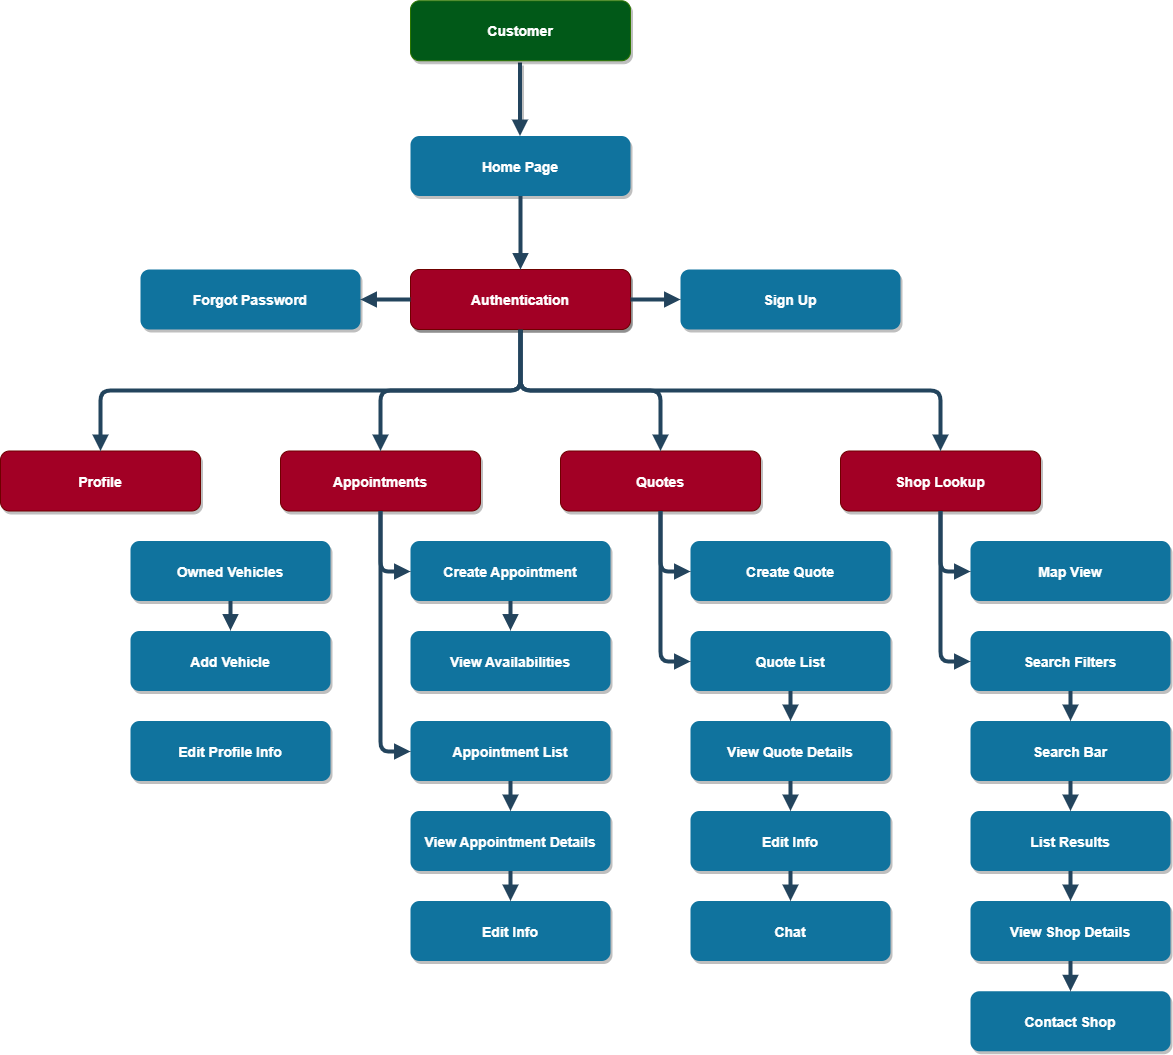
\includegraphics[scale=0.3]{SRS/customer_decomp.png}
    \caption{Customer Functional Decomposition Diagram}
    \label{fig:cfdf}
\end{figure}

\begin{figure}[H]
    \centering
    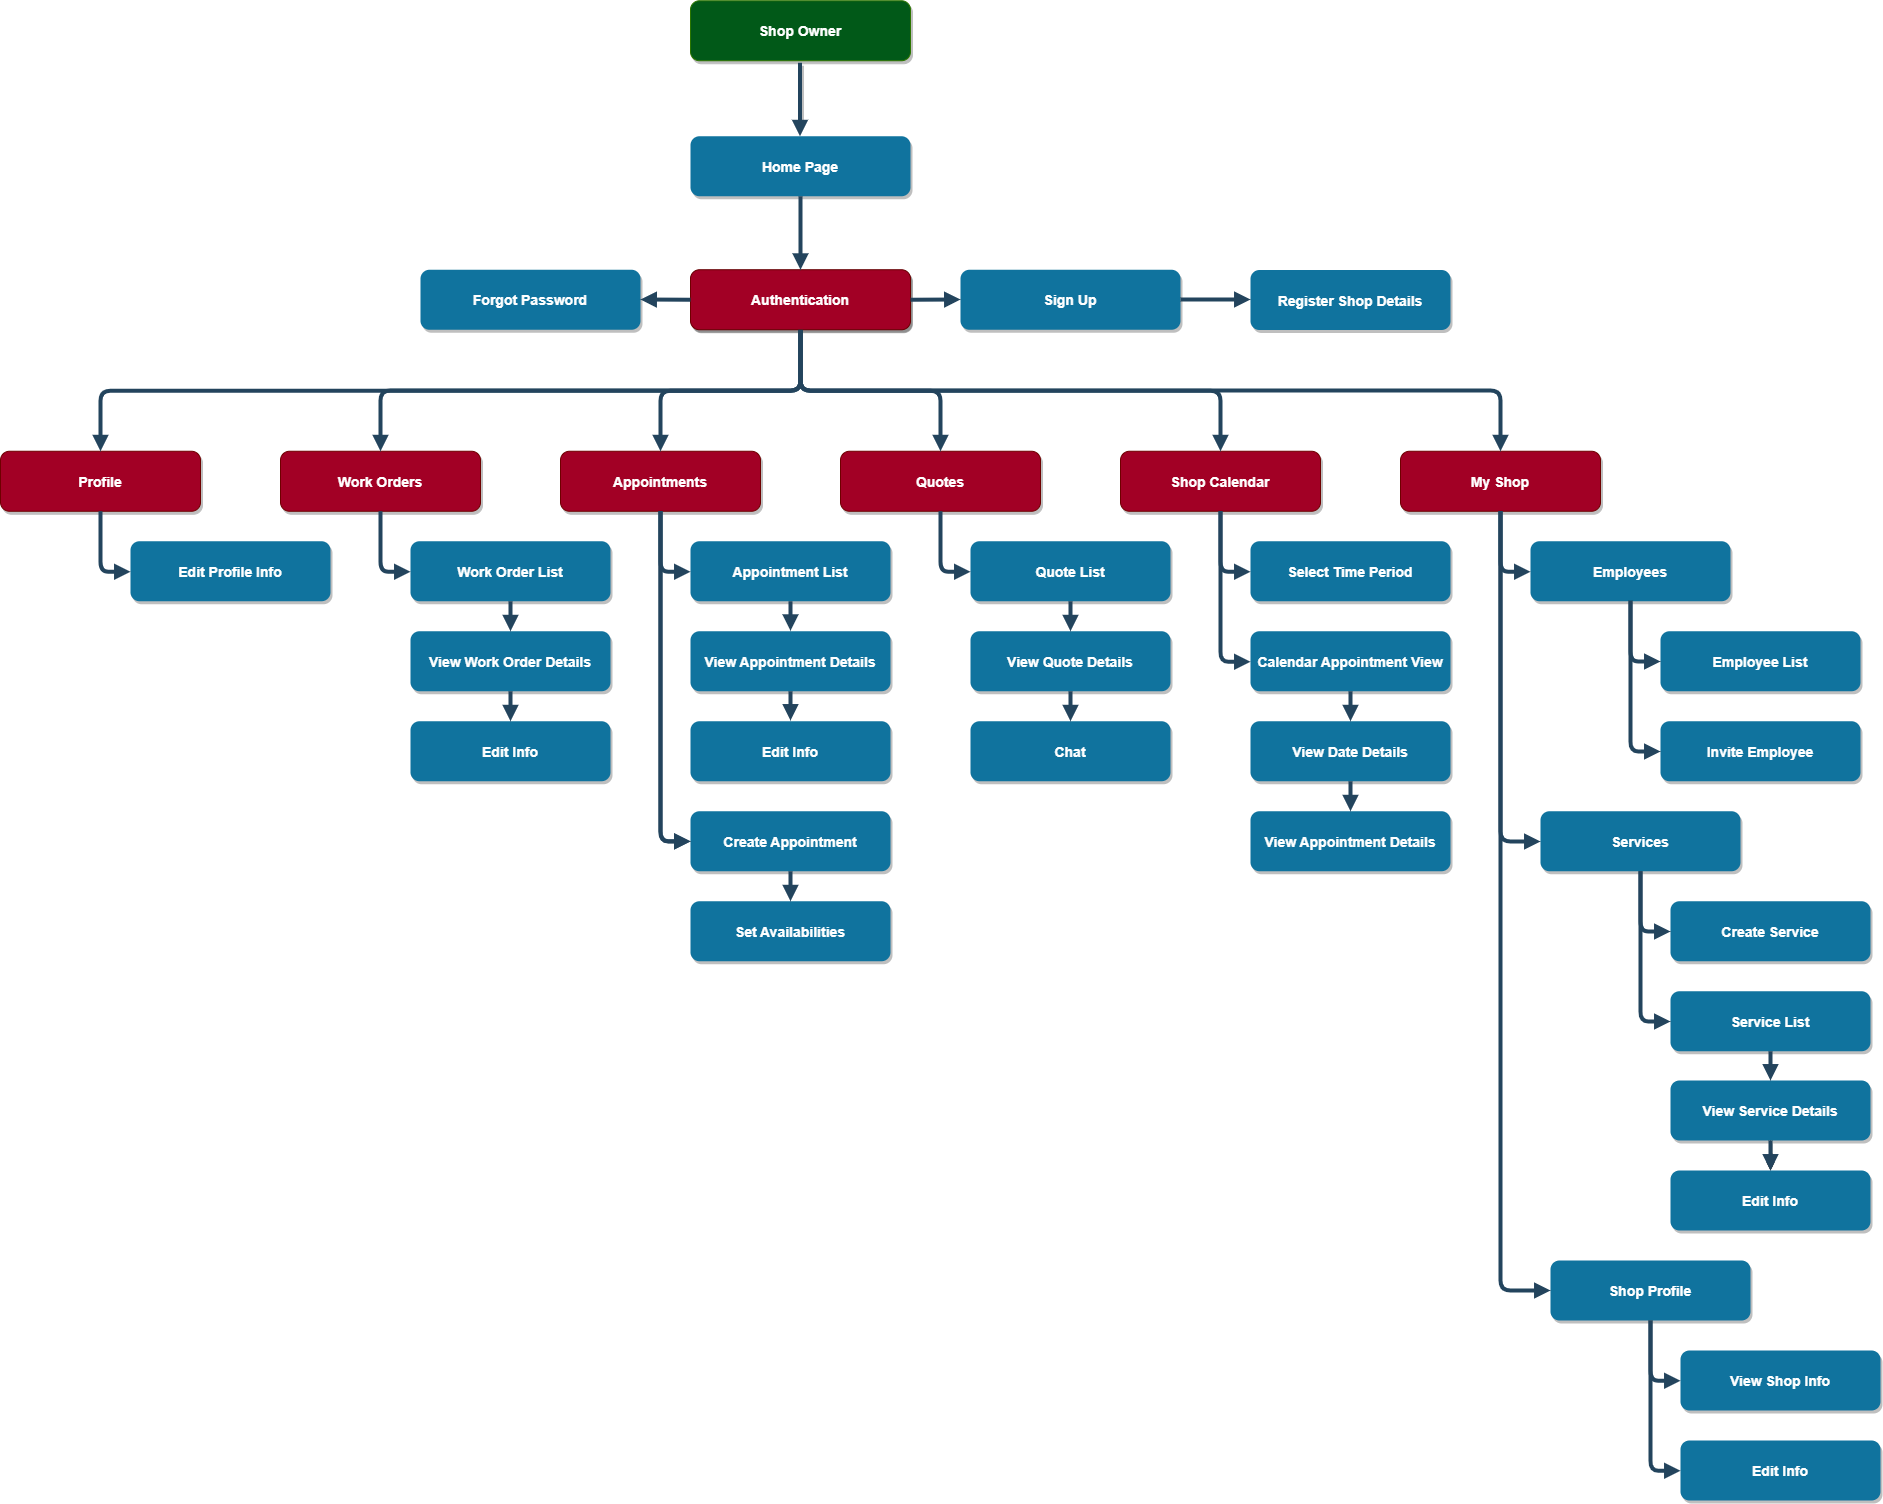
\includegraphics[scale=0.26]{SRS/owner_decomp.png}
    \caption{Shop Owner Functional Decomposition Diagram}
    \label{fig:ofdd}
\end{figure}

\begin{figure}[H]
    \centering
    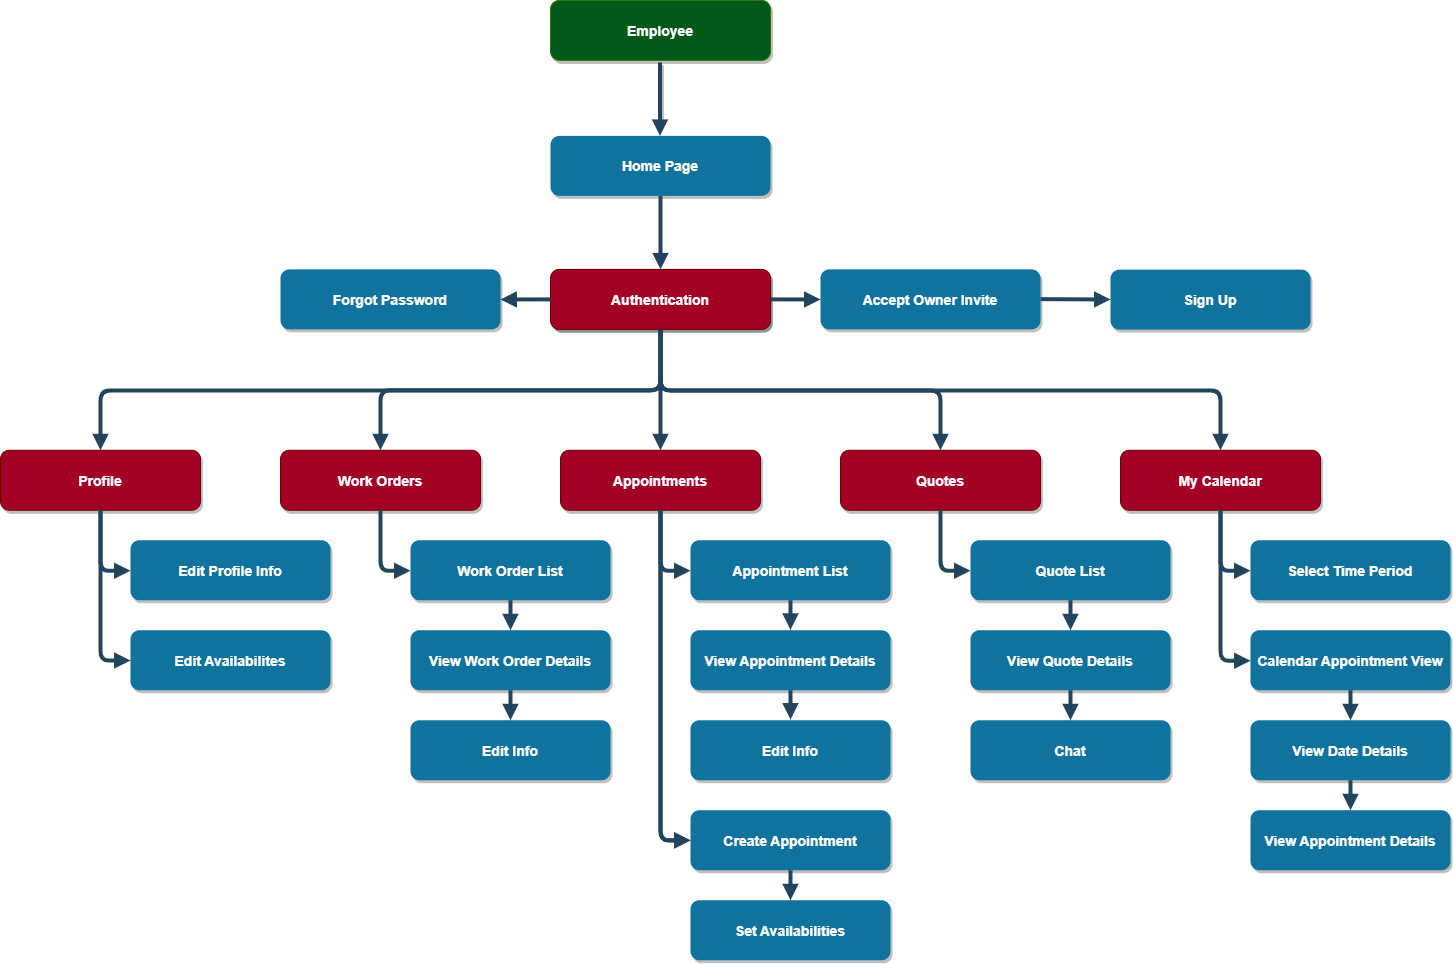
\includegraphics[scale=0.3]{SRS/employee_decomp.png}
    \caption{Employee Functional Decomposition Diagram}
    \label{fig:efdd}
\end{figure}

% Make these more specific and more measurable
\subsection{Nonfunctional Requirements}

\subsubsection{Look and Feel Requirements}

\begin {itemize}
\item[LFR\refstepcounter{lfrnum}\thelfrnum \label{R_Output}.] The system shall maintain a minimalist interface. Text information shall be concise and well-known iconography shall be used in place of text whenever applicable.\\
    Priority: High

\item[LFR\refstepcounter{lfrnum}\thelfrnum \label{R_Output}.] The system shall have components that create an illusion of depth based on gestalt design principles including colours, closure, and figure/ground.\\
    Priority: Medium
    
\item[LFR\refstepcounter{lfrnum}\thelfrnum \label{R_Output}.] The system shall have smooth transitions with animations after interactions to enhance both aesthetics and feedback for user input.\\
    Priority: Low
    
\item[LFR\refstepcounter{lfrnum}\thelfrnum \label{R_Output}.] The system shall have smoothed and rounded edges consistent with modern mobile application aesthetics instead of a box-like design.\\
    Priority: Low

\item[LFR\refstepcounter{lfrnum}\thelfrnum \label{R_Output}.] The system interface shall take on a consistent and limited colour palette (under 6 colours for functional or informative components such as buttons and text) to reduce visual clutter and reinforce signifiers.\\
    Priority: High
\end {itemize}

\subsubsection{Usability and Humanity Requirements}
\begin {itemize}
\item[UHR\refstepcounter{uhrnum}\theuhrnum \label{R_Output}.] The system shall be simple to use for someone with little technological background. Major functions for each user type shall be learnable in under 15 minutes for an average user with prior experience using a browser or mobile device.\\
    Priority: High
    
    \item[UHR\refstepcounter{uhrnum}\theuhrnum \label{R_Output}.] The system shall have support for accessibility. This would include making all features interactable with a screen reader. \\
    Priority: High
    
    \item[UHR\refstepcounter{uhrnum}\theuhrnum \label{R_Output}.] The system shall have emphasized interactive components. This should make forms the user can fill out, for example, have text fields that are easily identifiable as editable.\\
    Priority: Medium

    \item[UHR\refstepcounter{uhrnum}\theuhrnum \label{R_Output}.] The system shall attempt to minimize the number of clicks or taps per action.\\
    Priority: High

    \item[UHR\refstepcounter{uhrnum}\theuhrnum \label{R_Output}.] The system shall avoid forcing the user to input text, instead preferring selection from a list of options or auto-generation of required fields.\\
    Priority: Medium
\end {itemize}

\subsubsection{Performance Requirements}

\begin {itemize}
    \item[PR\refstepcounter{prnum}\theprnum \label{R_Output}.] The system shall be up and running 24/7 except for periodic monthly maintenance or unexpected server-hosting issues.\\
    Priority: High
    
    \item[PR\refstepcounter{prnum}\theprnum \label{R_Output}.] The system shall not require memory storage except for an automatic sign-in token.\\
    Priority: Medium
    
    \item[PR\refstepcounter{prnum}\theprnum \label{R_Output}.] The database get and update requests shall require less than 1 and 5 seconds respectively.\\
    Priority: High
\end {itemize}

\subsubsection{Operational and Environmental Requirements}

\begin {itemize}
    \item[OER\refstepcounter{oernum}\theoernum \label{R_Output}.] The product shall be available as a website.\\
    Priority: High
    
    \item[OER\refstepcounter{oernum}\theoernum \label{R_Output}.] The product shall work on latest versions of Chrome, Firefox, Edge, and Safari browsers as a website.\\
    Priority: High
    
   % \item[OER\refstepcounter{oernum}\theoernum \label{R_Output}.] The product shall work on latest versions of Apple iOS and Android as a mobile application.
\end {itemize}

\subsubsection{Maintainability and Support Requirements}

\begin {itemize}
    \item[MSR\refstepcounter{msrnum}\themsrnum \label{R_Output}.] The product shall have to be updated to work with latest versions of Chrome, Firefox, Edge, and Safari.\\
    Priority: High
    
    % \item[MSR\refstepcounter{msrnum}\themsrnum \label{R_Output}.] The product shall have a contact email for support.
\end {itemize}

\subsubsection{Security Requirements}

\begin {itemize}
    \item[SR\refstepcounter{srnum}\thesrnum \label{R_Output}.] The product shall securely store user information including passwords, and addresses using encryption.\\
    Priority: High
    
     \item[SR\refstepcounter{srnum}\thesrnum \label{R_Output}.] The product shall only allow the creator of a data node (shop, appointment, etc) to delete it.\\
     Priority: High
     
     \item[SR\refstepcounter{srnum}\thesrnum \label{R_Output}.] The product shall only allow a certain number of a specific database operation (sign-in attempt, chat message, create an appointment, etc) by a user every 15 seconds before the system will spawn a temporary timeout to avoid spamming attacks.\\
     Priority: High
\end {itemize}

\subsubsection{Cultural and Political Requirements}

\begin {itemize}
    \item[CPR\refstepcounter{cprnum}\thecprnum \label{R_Output}.] The product shall not use any language that could be offensive to some cultures.\\
    Priority: High
    
    \item[CPR\refstepcounter{cprnum}\thecprnum \label{R_Output}.] The product shall have functionality support for multiple languages if other languages than English are added to the translation configuration.\\
    Priority: Low
    
    \item[CPR\refstepcounter{cprnum}\thecprnum \label{R_Output}.] The product shall have a profanity filter for the chat system.\\
Priority: Low
\end {itemize}

\subsubsection{Compliance Requirements}

\begin {itemize}
    \item[CR\refstepcounter{crnum}\thecrnum \label{R_Output}.] The product shall clearly state that Sayyara is not responsible for anything that occurs during the chat, appointment, or work order process.\\
    Priority: Medium
\end {itemize}

\subsection{Likely Changes to Requirements}    

\begin {itemize}
    \item[LC\refstepcounter{lcnum}\thelcnum
    \label{R_Output}.] The product may not always continue to support browsers like Firefox.
    
    \item[LC\refstepcounter{lcnum}\thelcnum
    \label{R_Output}.] The product may switch to relying on an authentication system instead of an access token on mobile devices for vehicle owners.
    
    \item[LC\refstepcounter{lcnum}\thelcnum
    \label{R_Output}.] The product may require more maintenance periods in the future.
    
    \item[LC\refstepcounter{lcnum}\thelcnum
    \label{R_Output}.] The product may add other languagage translation configurations for support.
\end {itemize}

\subsection{Unlikely Changes to Requirements}    

\noindent \begin{itemize}

\item[UC\refstepcounter{ucnum}\theucnum\label{UC_meaningfulLabel}.] The application will be a PWA and must run on both desktop and mobile devices and this requirement will not change.

\item[UC\refstepcounter{ucnum}\theucnum\label{UC_meaningfulLabel}.] The application is meant to be designed for users who are not very tech savvy, so features will be simplistic and easy to navigate.

\item[UC\refstepcounter{ucnum}\theucnum\label{UC_meaningfulLabel}.] The intended users of the application are unlikely to change; the application is designed for autmotive shop owners, their employees, and their potential customers.

\item[UC\refstepcounter{ucnum}\theucnum\label{UC_meaningfulLabel}.] It is intended for the application to have a monthly subscription service for shop owners to host their shop and its services on the website.

\end{itemize}

%\subsection{Planned Implementation Schedule}

\newpage

\section{Project Issues}

\subsection{Open Issues}
\begin {itemize}
    \item Uncertainty in scope \\ 
    A potential issue is the uncertainty in project scope with respect to the 
    limited development time. In the initial meeting, the client envisioned an 
    expansive system with three main views to include the functionalities for 
    the three user groups: shop owners, employees, and customers. The main 
    functions in each component were assigned priority based on their inclusion 
    in the MVP. However, the team determined that the completion of all 
    currently labelled MVP functionality may be difficult due to the time 
    constraint of the February deadline. Further discussions will be conducted 
    with the client to adjust the MVP scope to adapt to this timeline.
    
    \item Payment system\\
    A subscription-based payment system is required for the commercial 
    distribution of the product. No payment options have been explored, and the 
    client is responsible for setting up the required banking and payment 
    routing. Whether the payment system or a mock-up of one should be 
    implemented in the MVP will be a topic of discussion with the client.
\end {itemize}

\subsection{Off-the-Shelf Solutions}

\subsubsection{Ready-Made Products}
A number of existing software offer scheduling, billing, and communication 
tools for auto service shops, covering some but not all of the client 
requirements.

\begin {itemize}
    \item Shop-Ware (\url{www.shop-ware.com}) \\ 
    Shop-Ware is a cloud-based auto shop management software with features such 
    as service analytics, quote generation, employee management, inventory 
    tracking, and digital vehicle inspection. The primary users are shop owners 
    and employees, and as such offers little utility to customers.
    
    \item AutoLeap (\url{www.autoleap.com}) \\
    Similar to Shop-Ware, AutoLeap markets itself as an auto shop workflow 
    optimization software, focusing on features such as inspection report, 
    estimates, invoice generation. It also provides customer-facing features 
    including automated scheduling and Google reviews. However, it is 
    shop-specific and does not feature a centralized hub for customers to 
    contact multiple service providers.
    
    \item Setmore (\url{www.setmore.com/industries/automotive})
    Setmore is a free auto service scheduling tool. Focusing primarily on 
    booking appointments, Setmore offers APIs to display a scheduling calendar 
    on auto shops' own websites, with additional features such as automated 
    mobile reminders. 
\end {itemize}

\subsubsection{Reusable Components}
    \begin{itemize}
        \item Front end components and styling can be built on top of existing 
        frameworks such as Bootstrap or MUI.
        \item Google Calendar API can be the basis of the scheduling 
        functionality.
        \item Mobile text notification can be accomplished using available 
        tools such as Twilio API.
    \end{itemize}

\subsection{New Problems}
While switching auto service-related interactions from the traditional 
in-person or phone methods to a centralized online platform will reduce overall 
effort by the customers, its use requires access to mobile or computer devices 
with Internet connections, as well as the basic knowledge of operating such 
devices. While these basic technological experiences have become near 
ubiquitous, it can still potentially preclude some users such as older 
employees or customers.

Shop owners and employees may also require time for the initial training or 
practice for using the application. The myriad of shop-facing functions imply 
that, even with an intuitive, user-friendly design, some acclimatization may 
still be required.

Additionally, the platform is only as responsive as the shops that it hosts. 
The asynchronous options of online communication may result in tardiness in 
shop-customer communications compared to traditional contact methods.



\subsection{Tasks}
\begin{itemize}
    \item Architectural design of the full application is expected to be 
    completed by October 20, 2022. 
    \item The full team will work on the customer, employee, and shop owner 
    views concurrently, with feature-based tasks assigned to individual members 
    according to expertise. Please refer to the Development Plan for a detailed 
    breakdown of the feature-branch workflow.
    \item A few core functions for each view will be implemented in a mock-up 
    back end, to be displayed on skeletal front end designs for the POC 
    demonstration by November 13.
    \item Additional features corresponding to the requirements are to be 
    implemented before February 3, 2023.
    \item Unit testing is carried out during the development of each feature. 
    While systematic testing is conducted monthly.
    \item Updates to the requirements and implementation are to be discussed 
    and formulated based on regular weekly meetings between the development 
    team and the client.
    
\end{itemize}

\subsection{Migration to the New Product}
The initial setup of the software requires the shop owners to register an 
account or profile for their shop, and perform owner-specific configurations 
such as granting access permissions to employees. The employees are required to 
install the software on their devices, and familiarize with use cases such as 
responding to scheduling requests, and preparing online service reports. The 
software is expected to work in tandem with traditional real time contact 
methods, and so does not replace phone or in-person contacts in the foreseeable 
future.

\subsection{Risks}
\begin{itemize}
    \item Due to limited time, the team will focus primarily on developing the 
    main features rather than application security. As such, the MVP may have 
    little protection against malicious security exploits.
    \item The development build will use mock data provided by the client. 
    There is a risk that the system may not scale up readily to accommodate 
    high-volume real traffic and data, as traffic-stress testing is beyond 
    purview of the MVP.
    \item The team consists of six developers of varying levels of experience 
    and areas of expertise. Consequently there exists the risk of stylistic 
    differences in different components of the application as a side effect of 
    the feature-branch workflow. Coding standards and the pull request review 
    process will alleviate some of the differences but full consistency may be 
    difficult to achieve during the short development period.
\end{itemize}

\subsection{Costs}

The permitted budget for the project is \$750. Being an entirely software 
project, the development cost of the project is expected to be small. The team 
plans to use free or low-cost hosting services to deploy the development build. 
The available budget may be used to purchase commercial framework or library to 
assist in the development.\\

Moreover, there is heavy emphasis on deploying and testing locally to further save on testing costs. These cost savings do not transfer to deployment when real customers start using the product, therefore the following estimates are highly variable and prone to noise.\\

\begin{table}
    \begin{tabularx}{\textwidth}{l X}
        \toprule
        \textbf{Service} & \textbf{Cost} \\
        \midrule
        Database Storage & \$0/month during development, Bundled in the server hosting costs\\
        Server Hosting & variable depending on usage, starts at \$10/month\\
        Website Domain Name & \$20/year\\
        \bottomrule
    \end{tabularx}
    \caption{Costs}
\end{table}


\subsection{User Documentation and Training}
N/A
\subsection{Waiting Room}
\begin{itemize}
    \item Auto service features that requires domain-specific knowledge such as 
    onboard diagnostic report are valuable extensions to the tool that can be 
    developed post-MVP.
    \item Customer and employee account features such as configurations and 
    customization are not a part of the MVP but should be included in future 
    builds.
    \item Artificial intelligence integration should be explored for features 
    such as quote generation, scheduling, and analytics.
\end{itemize}
\subsection{Ideas for Solutions}
N/A

\newpage
\section{Traceablity Matrices and Graphs}

    \begin{table}[h!]
        \centering
        \begin{tabular}{|c|c|c|c|c|c|c|c|c|c|}
            \hline
            &     G1&G2&G3&G4&G5&G6&G7&G8&G9\\ \hline
            UC1  &  & X&  &  &  &  &  &  & X\\ \hline
            UC2  &  &  &  & X&  &  &  &  & \\ \hline
            UC3  &  &  & X& X&  &  &  & X& \\ \hline
            UC4  &  &  &  &  &  &  & X&  & \\ \hline
            UC5  &  &  &  & X&  & X&  &  & \\ \hline
            UC6  &  &  &  &  & X& X&  & X& \\ \hline
            UC7  & X& X&  &  & X& X&  &  & \\ \hline
            UC8  & X& X&  &  &  &  &  &  & \\ \hline
            UC9  &  &  &  & X&  & X&  &  & X\\ \hline
            UC10 &  &  &  & X&  & X&  &  & \\ \hline
            UC11 &  &  &  & X&  & X&  &  & X\\ \hline
            UC12 & X& X&  & X& X&  &  &  & \\ \hline
            UC13 &  &  &  &  &  & X&  &  & X\\ \hline
            UC14 &  &  &  &  &  & X&  &  & X\\ \hline
            UC15 & X& X&  & X&  &  &  &  & \\ \hline
            UC16 &  &  X& &  &  &  &  &  & \\ \hline
            UC17 &  X& X& &  &  &  & X&  & X\\ \hline
            UC18 &  X& X& &  &  &  &  &  & X\\ \hline
            UC19 &  &  & X&  &  &  &  &  & X\\ \hline
            UC20 &  & X& X&  &  &  &  &  & X\\ \hline
        \end{tabular}
        \caption{Traceability Matrix between Goals and Use Cases}
    \end{table}

\newgeometry{top=0.2in,left=0.2in,right=0.2in,bottom=0.6in}
\begin{landscape}

    \begin{table}[h!]
        \centering
        \resizebox{\columnwidth}{!}{%
        \begin{tabular}{|c|c|c|c|c|c|c|c|c|c|c|c|c|c|c|c|c|c|c|c|c|}
            \hline
            &     UC1&UC2&UC3&UC4&UC5&UC6&UC7&UC8&UC9&UC10&UC11&UC12&UC13&UC14&UC15&UC16&UC17&UC18&UC19&UC20    \\ \hline
            AuR1 &  X&   &   &   &   &   &   &   &   &    &    &    &    &    &    &   X & & & &\\ \hline
            AuR2 &  X&   &   &   &   &   &   &   &   &    &    &    &    &    &    &   X & & & &\\ \hline
            AuR3 &  X&   &   &   &   &   &   &   &   &    &    &    &    &    &    &   X & & & &\\ \hline
            SR1  &   &   &   &   &   &   &   &  X&   &    &   X&   X&    &    &    &     & & & &\\ \hline
            SR2  &   &   &   &   &   &   &   &  X&   &    &   X&   X&    &    &    &     & & & &\\ \hline
            SR3  &   &   &   &   &   &   &   &   &   &    &    &    &    &    &    &     & & & &\\ \hline
            PAR1 &   &   &   &   &   &   &   &  X&   &    &    &    &    &    &    &     & & & &\\ \hline
            PAR2 &   &   &   &   &   &   &   &  X&   &    &    &    &    &    &    &     & & & &\\ \hline
            PAR3 &   &   &   &  X&   &   &   &   &   &    &    &    &    &    &   X&   X & & & &\\ \hline
            PAR4 &   &   &   &  X&   &   &   &  X&   &    &    &    &    &    &    &     & & & &\\ \hline
            PAR5 &   &   &   &   &   &   &   &   &   &    &    &    &    &    &    &     & & & &\\ \hline
            PAR6 &   &   &   &   &   &   &   &   &   &    &    &    &    &    &    &     & & & &\\ \hline
            PAR7 &   &   &   &   &   &   &   &   &   &    &    &    &    &    &   X&     & & & &\\ \hline
            PAR8 &   &   &   &   &   &   &   &   &   &    &    &    &    &    &    &     & & & &\\ \hline
            PAR9 &  X&   &   &   &   &   &   &   &   &    &    &    &    &    &    &   X & & & &\\ \hline
            PAR10&   &   &   &   &   &   &   &   &   &    &    &    &   X&   X&    &     & & & &\\ \hline
            PAR11&   &   &   &   &   &   &   &   &   &    &    &    &   X&   X&    &     & & & &\\ \hline
            % PAR12&   &   &   &   &   &   &   &   &   &    &    &    &   X&   X&   X&   & & & &  \\ \hline
            ApR1 &   &   &   &   &   &  X&  X&  X&   &    &    &    &    &    &    &     & & & &\\ \hline
            ApR2 &   &   &   &   &  X&  X&  X&   &   &    &    &    &    &    &    &     & & & &\\ \hline
            ApR3 &   &   &   &   &  X&  X&   &   &   &    &    &    &    &    &    &     & & & &\\ \hline
            % ApR4 &   &   &   &   &  X&  X&   &   &   &    &    &    &    &    &    &   & & & &  \\ \hline
            % ApR5 &   &   &   &   &   &  X&   &   &   &    &    &    &    &    &    &   & & & &  \\ \hline
            % WOR1 &   &   &   &   &   &   &   &   &  X&   X&    &    &    &    &    &   & & & &  \\ \hline
            % WOR2 &   &   &   &   &   &   &   &   &  X&   X&    &    &    &    &    &   & & & &  \\ \hline
            % WOR3 &   &   &   &   &   &   &   &   &  X&   X&    &    &    &    &    &   & & & &  \\ \hline
            QR1  &   &   &   &  X&   &   &   &   &   &    &    &    &    &    &    &     & & & &\\ \hline
            QR2  &   &   &  X&   &   &   &   &   &   &    &    &    &    &    &    &     & & & &\\ \hline
            % QR3  &   &  X&  X&   &   &   &   &   &   &    &    &    &    &    &    &   & & & &  \\ \hline
            % VR1  &   &   &   &   &   &   &   &   &   &    &    &    &    &    &    &   & & & &  \\ \hline
            % VR2  &   &   &   &   &   &   &   &   &   &    &    &    &    &    &    &   & & & &  \\ \hline
            SLR1  &   &   &   &   &   &   &   &   &   &    &    &    &    &    &    &    & X&  &  & \\ \hline
            SLR2  &   &   &   &   &   &   &   &   &   &    &    &    &    &    &    &    &  & X&  & \\ \hline
            SLR3  &   &   &   &   &   &   &   &   &   &    &    &    &    &    &    &    &  &  & X&\\ \hline
            SLR4  &   &   &   &   &   &   &   &   &   &    &    &    &    &    &    &    &  &  &  & X\\ \hline
            SLR5  &   &   &   &   &   &   &   &   &   &    &    &    &    &    &    &    &  &  &  & X\\ \hline
            SLR6  &   &   &   &   &   &   &   &   &   &    &    &    &    &    &    &    &  & X&  &\\ \hline
        \end{tabular}%
        }
        \caption{Traceability Matrix between Use Cases and Functional Requirements}
    \end{table}

\end{landscape}
\restoregeometry

    \begin{table}[h!]
        \centering
        \begin{tabular}{|c|c|c|c|c|c|c|c|c|c|}
            \hline
            &    G1&G2&G3&G4&G5&G6&G7&G8&G9 \\ \hline
            LFR1&  & X&  &  &  &  &  &  & X\\ \hline
            LFR2&  &  &  &  &  &  &  &  & X\\ \hline
            LFR3&  & X&  &  &  &  &  &  & X\\ \hline
            LFR4&  & X&  &  &  &  &  &  & X\\ \hline
            LFR5&  &  &  &  &  &  &  &  & X\\ \hline
            UHR1&  & X&  &  &  &  & X&  & X\\ \hline
            UHR2& X&  &  & X&  &  & X&  & X\\ \hline
            UHR3&  &  &  &  &  &  &  &  & X\\ \hline
            UHR4&  &  &  &  &  &  &  &  & X\\ \hline
            UHR5& X& X&  & X&  & X&  & X& X\\ \hline
            PR1 & X& X&  &  &  &  & X&  & X\\ \hline
            PR2 &  &  &  &  &  &  &  &  & X\\ \hline
            PR3 &  & X&  &  &  &  &  &  & X\\ \hline
            OER1& X& X&  & X& X&  &  &  & X\\ \hline
            OER2& X&  &  &  &  &  & X&  & X\\ \hline
            OER3& X&  & X&  &  &  & X&  & X\\ \hline
            MSR1&  &  &  &  &  &  &  &  & X\\ \hline
            % MSR2&  &  &  &  &  &  &  &  & X\\ \hline
            SR1 &  & X&  & X&  &  &  & X& X\\ \hline
            SR2 &  &  &  & X&  &  &  & X& X\\ \hline
            SR3 &  &  &  &  &  &  &  &  & X\\ \hline
            CPR1& X&  & X&  &  &  &  &  & X\\ \hline
            CPR2& X&  &  & X&  &  & X& X& X\\ \hline
            CPR3&  &  &  &  &  &  & X&  & X\\ \hline
            CR1 &  &  &  &  &  &  &  &  &  \\ \hline
        \end{tabular}
        \caption{Traceability Matrix between Goals and Non-Functional Requirements}
    \end{table}

\newpage{}
\section*{Appendix --- Reflection}

The team will collectively need to acquire and hone a variety of skills, 
technical and otherwise, in order to successfully complete this project. The 
implementation of the full stack application will require fluency in languages 
such as Python, Javascript, HTML, and CSS, as well as applicable packages and 
frameworks such as NodeJS, ReactJS, and databases. For a commercially 
marketable product, the team will also need to practice concepts such as 
user-centered design in UI/UX. 

Beyond technical skills, the team will learn to work together on a strict 
timeline through project management, communication, and constructive feedback. 
Such communication can include writing project documents, annotating the code, 
and providing or receiving feedback at regular meetings. The delivery of the 
final product arguably depends more on successful and consistent teamwork 
rather than individual technical skills.


\begin{itemize}
    \item Alyssa Tunney\\
        During my work term I had the opportunity to learn about full stack web development. During this time, I developed front end skills using JavaScript and the React framework. I also had the opportunity to extensively work with Python for both the back end of the web application and also had the opportunity to use it to automate tasks to triage a continuous integration system. One aspect of full stack web development that I would like to acquire more experience and knowledge in is database management. A lot of databases I was working with were already created so I just needed to write simple SELECT queries and so I would like to acquire more knowledge in the creation of databases and the relationships between them. These databases were SQL-based, so learning more about no-SQL databases is something I am interested in as well. I plan to research side-projects that incorporate a database management system. I also plan to research online courses that can teach me more about databases. Since I learn best by doing, I plan to pursue a side-project that incorporates a database management system so I can get hands-on experience that will be memorable and beneficial to this capstone project.
    \item Kai Zhu\\
        I have worked in full stack development and currently have experience
         in web technologies such as Node, React as well as other application 
         designs using C\# and Python. An avid believer of learning-by-doing, I 
         am interested to gain additional familiarity in industry development 
         environment by working on this project using practices such as CI/CD 
         and the feature-branch workflow.
    \item Christopher Andrade \\
        I currently have skills in front-end development using JavaScript, HTML, CSS, and frameworks like React, Redux, Sass, and more. Mostly, my skills pertain to user interface design. I now plan on learning Python back end skills to create a web server with authentication, and query data in a database, as these skills will be required for the project. These are things I haven't done much before. In order to do this, I will reach out to colleagues of mine who are familiar in Python back end and database management, and I will also be doing tiny small projects/challenges on the side with the help of online video tutorials to learn more. The latter will be what I pursue, because in the past I learned the basics of JavaScript needed to make a front end app using that method. 
    
    \item Harsh Gupta \\
        I have had experience in building and deploying high performance webapps at Tesla during my previous internship, where I leveraged NextJS and Python to create highly configurable static website generator with online content search functionality. Moreover, I have had experience in front-end development with TypeScript and React. This is especially important as the future platform of web is being build with frameworks like React. I plan on writing more applications around the recent breakthrough of LLM's(Large Language Models) and diffusion networks.

    \item Ethan Vince-Budan \\
        I currently do not have any experience with full stack development, although I do have some experience with languages and frameworks which may come in handy during this project. I have in the past worked on many standalone projects written in Python, Java, C, and some Lua. These projects are generally hosted on platforms which make use of git, which I have used for version control, issue tracking and a limited amount of CI/CD. Evidently I have a lot to learn about front-end development using React, which I intend to learn through online courses and forums such as Stack Overflow as I enjoy self-directed learning and experimentation. I predict that the back end workflow will be easier for me to adapt to as I have way more experience with related tech.

    \item Collin Kan \\
        I have had a lot of experience with full stack development. My experience started when I joined the DeltaHacks club here at McMaster as part of the technical team.. I was on the team for just shy of 2 years. I had to use Vue.Js, TypeScript, and Firebase (NoSQL) as part of the tech stack. I also had spent some time there designing easy to use interfaces as there would be hundreds af applicants using the application we were creating and maintaining. I also gained a good deal of experience working with the back end as part of my 12 month co-op. I used Go in order to create new APIs as well as update old, existing ones. During my 3 month co-op at Amazon, I was using TypeScript exclusively and had experience eliciting requirements, creating and writing design documents, as well as building an internal tool from he ground up using cloud (AWS) technologies, namely Lambda, DynamoDB, Step Functions, and CloudWatch/EventBridge. Outside of all this, I already had experience with Python while doing personal projects, coursework, and is my preferred programming language. Overall, I think I am well equipped with the necessary skillset in order to successfully complete this capstone project.
\end{itemize}



\end{document}